Tunel $ \Tau $ v molekule je v našem případě modelován posloupností koulí o různých poloměrech umístěných v prostoru. Pro posloupnost koulí $ \Tau = \{S_i\}_{i=0}^{n} $ navíc platí $ S_i \bigcap S_{i+1} \neq \emptyset $ pro všechna $ 0 \leq i < n $.
Pro představu jak takový tunel může vypadat uvádíme obrázek \ref{fig:basic_tunnel}.
\begin{figure}
  	\centering
	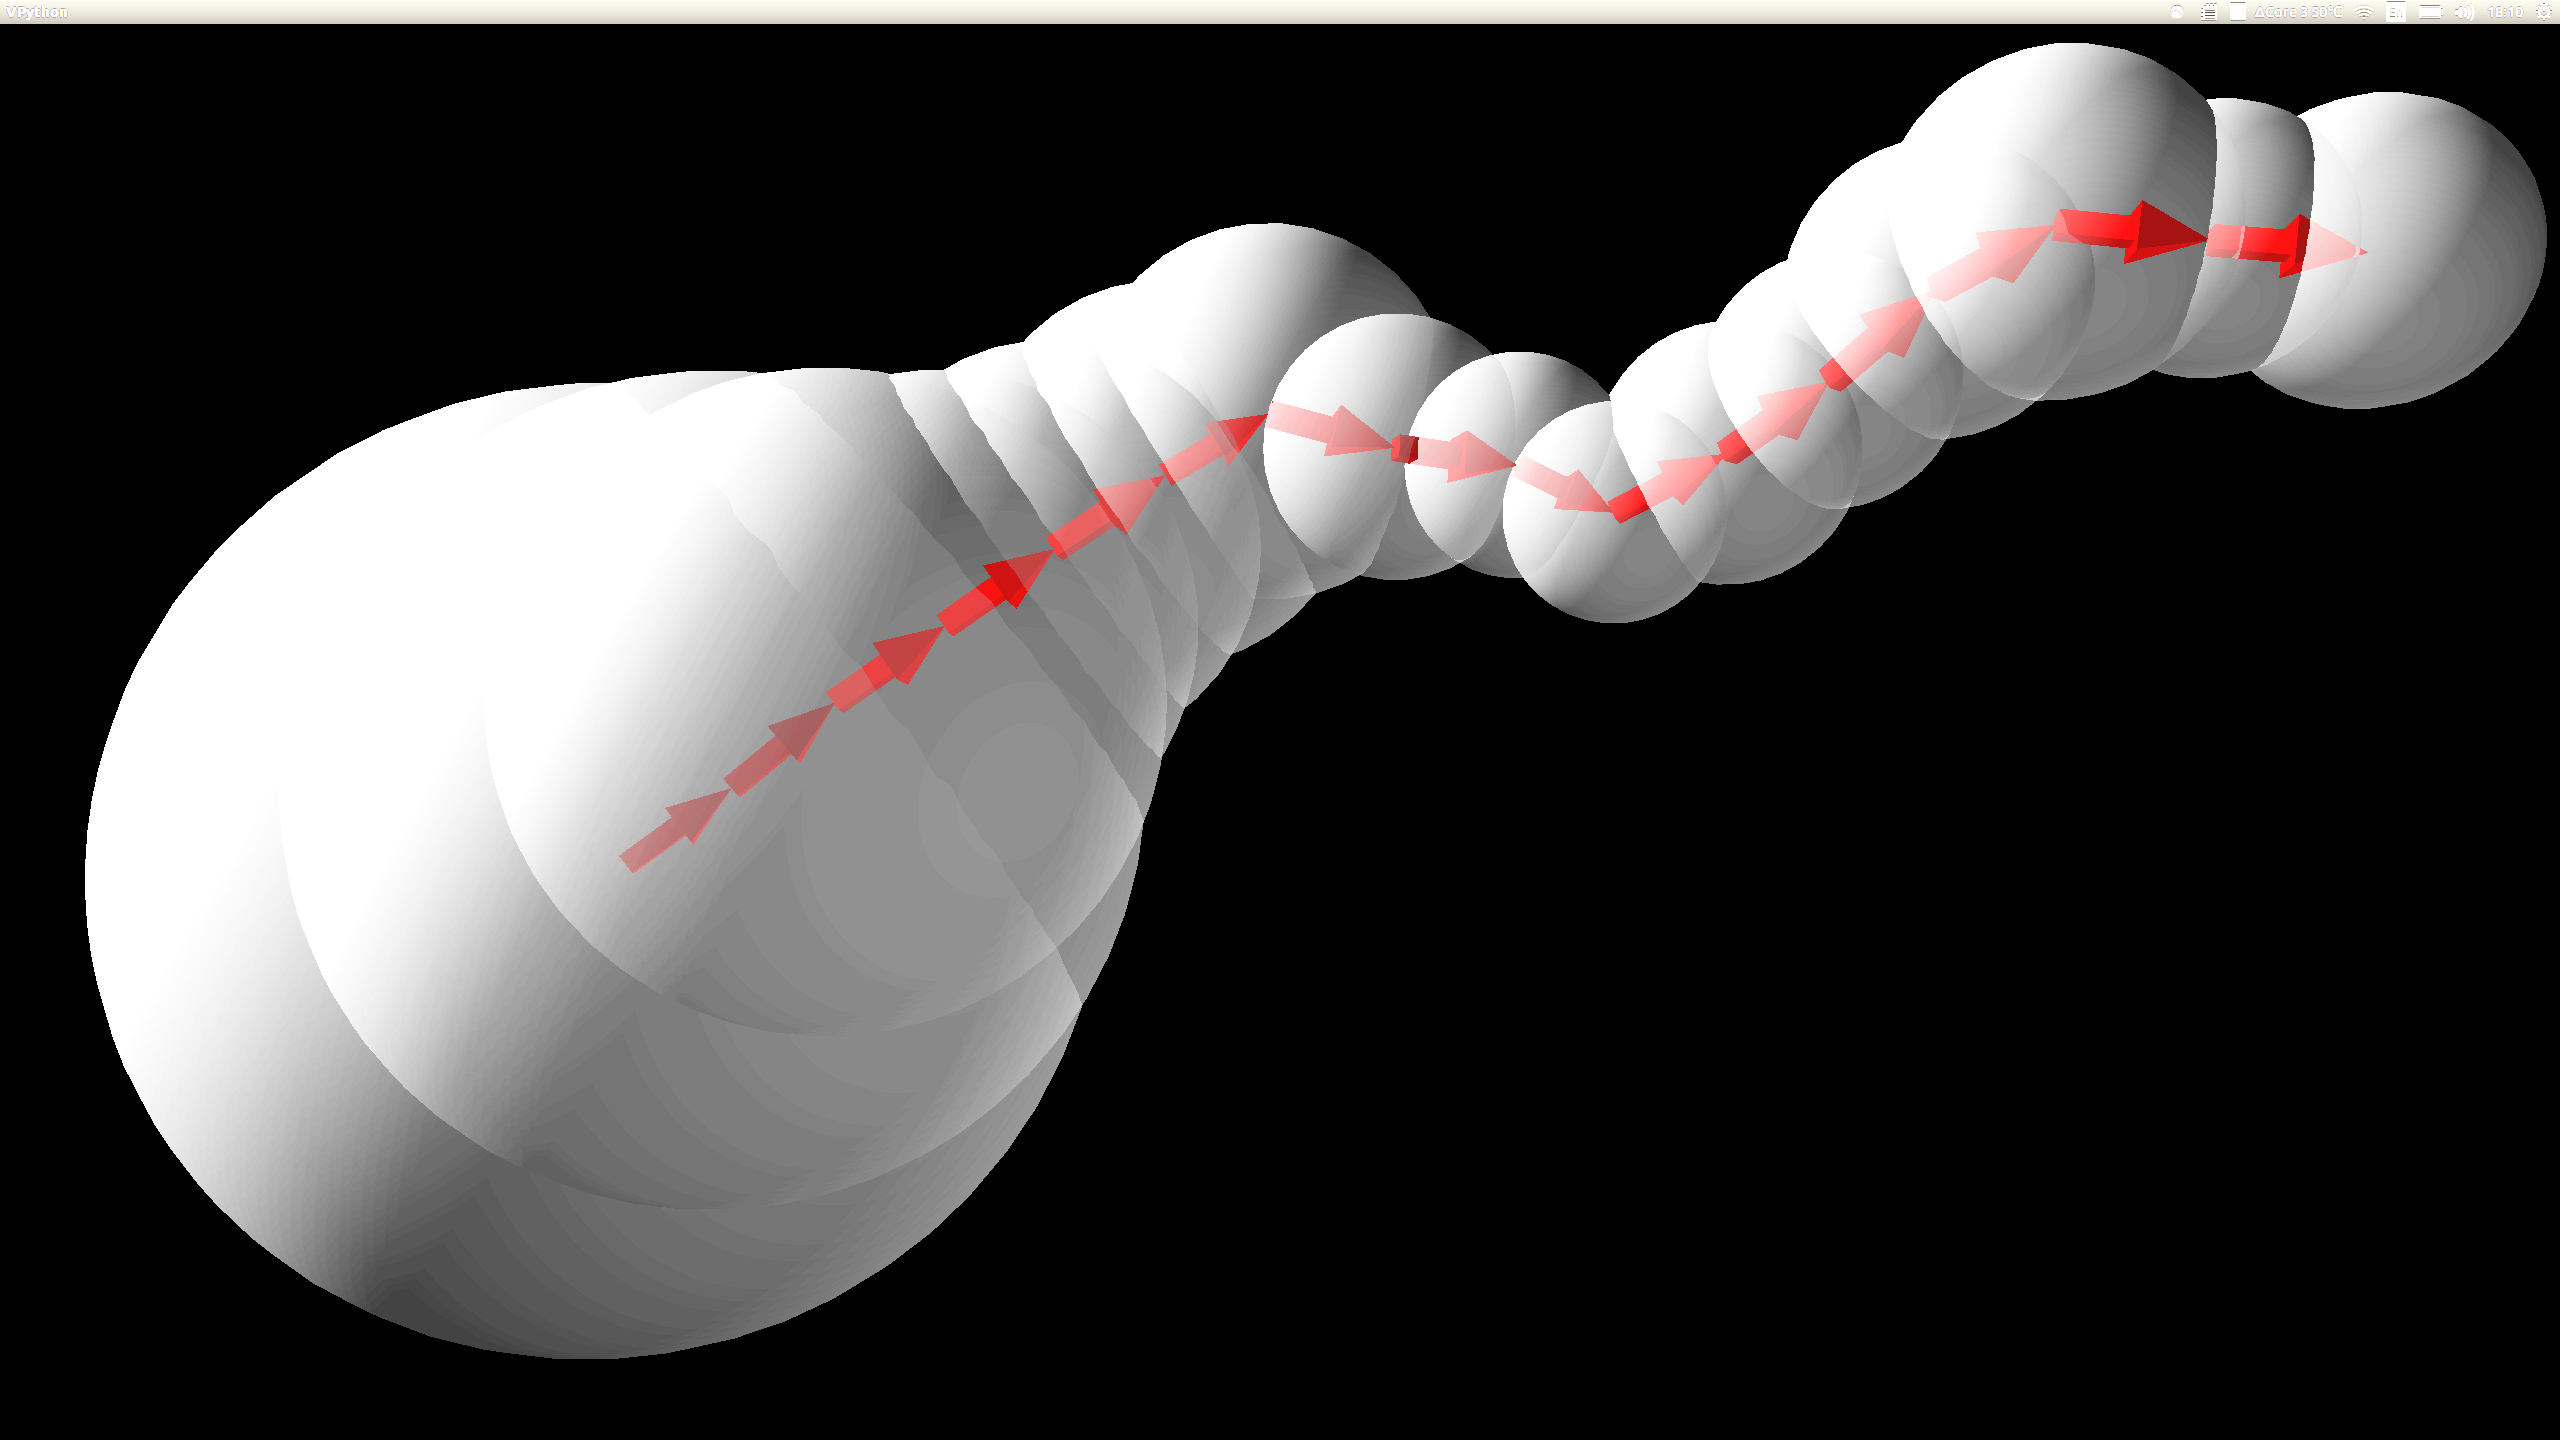
\includegraphics[width=100mm]{img/basic_tunnel.jpg}
	\caption{Sample of molecule tunnel}
  \centering
  \label{fig:basic_tunnel}
\end{figure}

Abychom mohli provádět docking ligandu, musíme nejprve takto definovaný tunel nařezat na jemné plátky - kruhy, na které pak v průběhu výpočtu budeme dokovat průběžné konformace ligandu. Popišme si nyní, jak by takové řezy měly vypadat.

\begin{defi}
Řezem tunelu $ \Tau $ rozumíme kruh v prostoru, který je určen uspořádanou trojicí $\theta = (A, u, r)$, kde $ A $ je střed, $ u \in \mathbb{R}^3 $ je normálnový vektor a $ r > 0 $ je poloměr.
Pro tento kruh $ \theta $ navíc musí platit, že $ \Tau \cap \theta $ je souvislá množina a navíc
$ r $ je nejmenší takové, že $ \theta \supseteq \Tau \cap \rho(\theta) $, kde $ \rho(\theta) $ značí rovinu určenou normálovým vektorem kruhu $ \theta $.
\end{defi}

\end{document}
